\section{Forwards, futures and options, and the cost of carry}

\begin{qfdefinition}[Derivative contracts: spot, forward, futures and options; payoffs, rights and obligations, exercise styles, futures specification and convergence]\label{def:derivative-contracts}
\qffield{Statement} A derivative ``involves two parties agreeing to a future transaction''; its value depends on the values of underlying variables, very often traded asset prices \citep[chap.~1, ``Introduction'', p.~23]{s7-hulloptions}. Hull's basic contracts:
\begin{itemize}
\item a \emph{spot contract} buys or sells an asset almost immediately; a \emph{forward contract} buys or sells it at a certain future time for a certain price, the delivery price $K$, and trades over the counter. The long side agrees to buy and the short side to sell (sec.~1.3, p.~28). At maturity the payoff per unit is $S_T-K$ to the long and $K-S_T$ to the short, where $S_T$ is the spot price; because it costs nothing to enter a forward, the payoff is also the total gain or loss (p.~29);
\item a \emph{futures contract} is the same kind of agreement, standardised and normally traded on an exchange, with the exchange clearing house standing between the parties (sec.~1.4, p.~30). Most positions are closed out by the opposite trade before delivery, but ``it is the possibility of final delivery that ties the futures price to the spot price'' (sec.~2.1, pp.~47--48);
\item an \emph{option}: a \emph{call} ``gives the holder the right to buy'' and a \emph{put} ``the right to sell'' the underlying asset by a certain date for the strike price. \emph{American} options can be exercised at any time up to expiration, \emph{European} options only on the expiration date. The holder has a right, not an obligation, and pays for it; forward and futures holders are obliged to buy or sell and pay nothing to enter apart from margin (sec.~1.5, p.~31).
\end{itemize}
The exchange specifies a futures contract's asset (with acceptable grades), contract size, delivery place and period, last trading day and price quotation; when alternatives are allowed, the short side usually chooses and files a notice of intention to deliver (sec.~2.2, pp.~48--50). For most contracts the exchange also sets daily price limits, after which trading normally stops for the day, though the exchange can change them; it also sets position limits for speculators (p.~50).

\qffield{Notation} $S_T$ spot price at maturity; $K$ delivery (forward) or strike (option) price; for a European call the payoff is $\max(S_T-K,0)$ and for a put $\max(K-S_T,0)$ (interpretation of Hull's definitions; the writer's payoffs are the negatives). \emph{Profit} is payoff less the premium paid, with the premium's time value ignored, as Hull does in his footnote (p.~32, n.~5).

\qffield{Conditions} \emph{Convergence.} As the delivery period approaches, the futures price converges to the spot price of the deliverable asset (sec.~2.3, pp.~50--51; Figure~\ref{fig:futures-convergence}). If futures traded above spot during delivery, shorting futures, buying the asset and delivering would profit; if below, buyers who want the asset would go long and take delivery. Interpretation: the argument needs the asset delivered to be the asset priced as spot, at the delivery location and grade, and delivery to be possible; cash-settled contracts converge through their final settlement rule instead, and when the short side chooses grade, place or timing, the futures price tracks the alternative it is expected to choose; Hull treats the timing choice in sec.~5.13 (p.~144).

\emph{Forward and futures} differ in standardisation, a single date against a range, settlement at the end against daily settlement, and credit risk (Table~2.3, p.~65); a forward gain is realised at maturity, a futures gain day by day (pp.~64--65).
\begin{figure}[ht]
\centering
% compendium/volatility-options/figures/futures-convergence.tikz
% Schematic drawn for slice 31 (2026-10-15) after the idea of Hull's Figure 2.1 (11th Global ed., p. 51); the curves
% are illustrative, not data. The legacy PNG it replaces is kept in notes/artefacts/volatility-options/figures/.
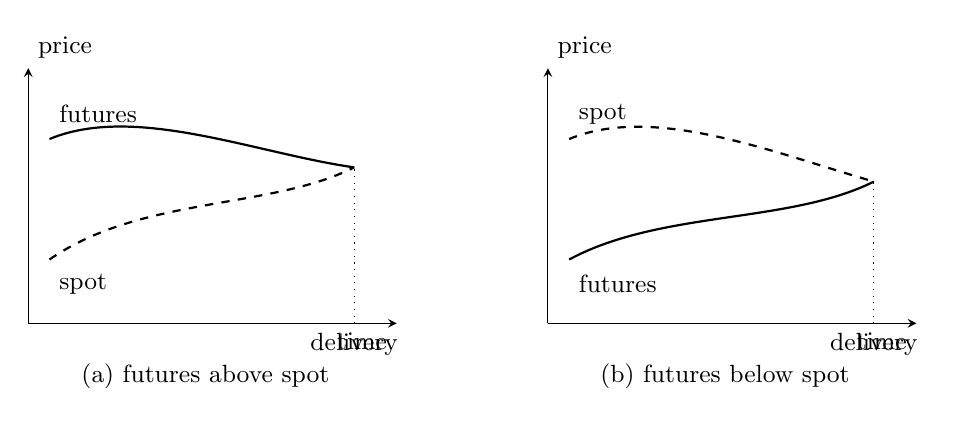
\begin{tikzpicture}[>=stealth, x=0.9cm, y=0.9cm, font=\small]
  \begin{scope}
    \draw[->] (0,0) -- (5.2,0) node[below left] {time};
    \draw[->] (0,0) -- (0,3.6) node[above right] {price};
    \draw[thick] (0.3,2.6) .. controls (1.5,3.1) and (3.2,2.4) .. (4.6,2.2);
    \draw[thick, dashed] (0.3,0.9) .. controls (1.6,1.8) and (3.4,1.6) .. (4.6,2.2);
    \node[right] at (0.3,2.95) {futures};
    \node[right] at (0.3,0.55) {spot};
    \draw[dotted] (4.6,0) -- (4.6,2.2); \node[below] at (4.6,0) {delivery};
    \node at (2.5,-0.75) {(a) futures above spot};
  \end{scope}
  \begin{scope}[xshift=6.6cm]
    \draw[->] (0,0) -- (5.2,0) node[below left] {time};
    \draw[->] (0,0) -- (0,3.6) node[above right] {price};
    \draw[thick, dashed] (0.3,2.6) .. controls (1.5,3.1) and (3.2,2.4) .. (4.6,2.0);
    \draw[thick] (0.3,0.9) .. controls (1.6,1.6) and (3.4,1.4) .. (4.6,2.0);
    \node[right] at (0.3,2.95) {spot};
    \node[right] at (0.3,0.55) {futures};
    \draw[dotted] (4.6,0) -- (4.6,2.0); \node[below] at (4.6,0) {delivery};
    \node at (2.5,-0.75) {(b) futures below spot};
  \end{scope}
\end{tikzpicture}

\caption{Convergence of the futures price to the spot price of the deliverable asset as delivery approaches; schematic after Hull, Figure~2.1, p.~51.}\label{fig:futures-convergence}
\end{figure}

\qffield{Practice} Checked with Hull's examples: a long six-month forward on \textsterling1 million at 1.2230 is worth $+\$77{,}000$ if spot ends at 1.3000 and $-\$23{,}000$ at 1.2000 (p.~29). One Apple December call contract on 100 shares, strike \$340, bought for \$2{,}030, pays $100\times(400-340)=\$6{,}000$ if exercised at \$400, a profit of \$3{,}970; one September put written at \$12.70 (\$1{,}270 received), strike \$290, exercised at \$250, costs \$4{,}000, a loss of \$2{,}730 (p.~32). Daily settlement and margin are in \hyperref[mech:futures-margin-settlement]{futures margin and settlement}; pricing in \hyperref[res:cost-of-carry-forward-price]{the cost of carry}.

\qffield{Pitfalls} The simplified definitions reversed the option rights: they gave a call the right to sell and a put the right to buy. Hull's is the opposite (p.~31). The ``derivatives market is much larger than the stock market in terms of underlying assets'' is Hull's statement (p.~23), but the size is a notional principal, not a value: Hull gives \$558.5 trillion of OTC notional against a gross market value of about \$11.6 trillion in December~2019 (pp.~27--28). Daily price limits, delivery terms and grades are contract-specific exchange rules, not universal features; Hull's examples are CME Group and ICE contracts as of 2021, and Hull notes that whether limits are on balance good is ``controversial'' (p.~50).

\qffield{See also} \hyperref[res:cost-of-carry-forward-price]{cost-of-carry forward price}; \hyperref[mech:futures-margin-settlement]{futures margin and settlement}; \hyperref[res:synthetic-short-put-call]{synthetic short through options} (put--call combinations as forwards); \hyperref[mech:otc-clearing-collateral]{OTC clearing and collateral}.

\end{qfdefinition}

\begin{qfresult}[Cost-of-carry forward price: no-arbitrage forward prices with income, yield and storage, the value of an existing forward, and the limits for consumption assets]\label{res:cost-of-carry-forward-price}
\qffield{Statement} For an \emph{investment asset}, one held solely for investment by at least some traders, with continuously compounded risk-free rate $r$ to maturity $T$ \citep[chap.~5, ``Determination of Forward and Futures Prices'', secs.~5.1--5.6, pp.~124--132]{s7-hulloptions}:
\[ F_0=S_0e^{rT}\ \text{(no income)},\qquad F_0=(S_0-I)e^{rT}\ \text{(income with present value $I$)},\qquad F_0=S_0e^{(r-q)T}\ \text{(yield $q$)}. \]
If $F_0$ is above the bound, buying the asset with borrowed money and selling forward locks in a profit; if below, shorting the asset (or, if shorting is impossible, selling it from holdings) and buying forward does (pp.~127--131). A long forward with delivery price $K$ agreed earlier is worth $f=(F_0-K)e^{-rT}$, for investment and consumption assets alike (sec.~5.7, p.~133). Special cases: a stock index with dividend yield $q$ (index arbitrage, sec.~5.9, pp.~135--137); a currency, with the foreign risk-free rate $r_f$ as the yield, $F_0=S_0e^{(r-r_f)T}$, interest rate parity (sec.~5.10, pp.~137--140); a commodity that is an investment asset, with storage cost net of income $U$ in present value, $F_0=(S_0+U)e^{rT}$, or $u$ as a proportion of price, $F_0=S_0e^{(r+u)T}$ (sec.~5.11, pp.~141--142).

The cost of carry $c$, storage plus financing less income, gives $F_0=S_0e^{cT}$ for an investment asset (sec.~5.12, pp.~143--144).

\qffield{Notation} $S_0$ spot price; $F_0$ forward (or futures) price; $r$ the $T$-year zero rate, continuously compounded; $q$ average yield over $T$; $U$, $u$ storage cost net of income; $y$ convenience yield; $c$ cost of carry ($r$ for a non-dividend stock, $r-q$ for an index, $r-r_f$ for a currency, $r-q+u$ for a commodity with income and storage, p.~144). Here $S_0$ and $F_0$ for a currency are dollars per unit of foreign currency (p.~138).

\qffield{Conditions} The derivation assumes that \emph{some} participants, such as large dealers, trade without transaction costs, pay the same tax rate on all net trading profits, borrow and lend at the same risk-free rate, and take arbitrage opportunities as they arise (sec.~5.3, p.~126). For a \emph{consumption asset}, held to be used rather than as an investment, the second arbitrage fails: owners will not sell the commodity to buy futures, so only $F_0\le(S_0+U)e^{rT}$ or $F_0\le S_0e^{(r+u)T}$ holds. The convenience yield $y$ is defined to close the gap, $F_0e^{yT}=(S_0+U)e^{rT}$, so that $F_0=S_0e^{(c-y)T}$; it is zero for investment assets (pp.~142--144).

Forward and futures prices are equal in theory when the short rate is constant or a known function of time; with random rates, futures exceed forwards when the asset is positively correlated with rates and fall below them when negatively correlated, differences Hull finds small for contracts of a few months (sec.~5.8, p.~135). Index arbitrage failed on 19--20 October 1987, when order delays and program-trading restrictions left December S\&P~500 futures up to 18 percent below the index (Business Snapshot~5.4, p.~137).

\qffield{Practice} Checked with Hull's examples: $40e^{0.05\times0.25}=40.50$ (p.~128); $(900-40e^{-0.03/3})e^{0.04\times0.75}=886.60$ (p.~131); $(50-2.162)e^{0.08\times10/12}=51.14$ (p.~132); with 2 percent paid once in six months, $q=2\ln1.02=3.96$ percent and $F_0=25e^{(0.10-0.0396)\times0.5}=25.77$ (p.~132); $f=(26.28-24)e^{-0.05}=2.17$ (p.~133); $0.7500e^{(0.01-0.03)\times2}=0.7206$ USD per AUD (p.~139); $(450+2e^{-0.07})e^{0.07}=484.63$ (p.~141). When short sales are impossible the arbitrage against a forward that is too low still works through holders who sell the asset and buy forward (pp.~129 and~131).

\qffield{Pitfalls} For consumption commodities only the upper arbitrage bound holds, and the convenience-yield sentence (``reflects market expectation on future availability'') is Hull's (p.~143) but applies to consumption assets only. The ``when a forward contract is first entered, the value is close to zero'' is Hull's opening sentence (p.~133); Hull adds that $K$ is set equal to the forward price, so $f=0$ at inception, . Its currency formula defined $S_0$ as ``price of local currency in foreign currency''; in Hull both $S_0$ and $F_0$ are the domestic price of one unit of foreign currency, with $r$ domestic and $r_f$ foreign, and many market quotes run the other way (p.~138). Borrowing constraints, borrow fees and recall, which make shorting costly, are in \hyperref[def:securities-lending-fee-rebate]{lending fees and rebates}.

\qffield{See also} \hyperref[def:derivative-contracts]{derivative contracts}; \hyperref[def:arbitrage]{arbitrage} (carrying costs and bounds in Harris's terms); \hyperref[mod:minimum-variance-hedge-ratio]{minimum-variance hedge ratio}; \hyperref[def:futures-hedge-basis]{futures hedges and basis}.

\qffield{Further reading} The theory of storage and convenience yields belongs to the commodity pathways.

\end{qfresult}
